\section{Case Study} \label{sect:case-study}
% > Introduction to Case Study

% What is USNO-B1.0?
% \usno is an all-sky catalog composed from multiple sky surveys during the interval from 1949 to 2002 \cite{web:caltech:usno} that indicates positions, proper motions, star/galaxy estimators and other astronomical features for 1,042,618,261 objects derived from 3,643,201,733 distinct observations \cite{web:ap-i:usno}.

% TODO: What is Pan-STARRS1?

% > Overall idea of the case study

% Architecture overview
\section{Architecture} \label{sect:case-study:arch}

% Introduction to overall architecture 
% Why two separate applications?
The following section motivates and outlines the architecture choices made in order to create the tools required to conduct the case study. The software required to perform the case study is split into two independent applications. The first application focuses in user interaction and experience, referred to as the \mlblink User Interface (\mlblinkui), and the second one is in charge of dealing with business logic and providing the required resources to the \mlblinkui, referred to as the \mlblink Application Programming Interface (\mlblinkapi). Through out the report, these two applications are also described as the client and server respectively.  \newline

While the two applications could have been developed as a monolith, having two decoupled applications allows to clearly distinguish between client responsibilities and business logic. On the other hand, splitting the project into two separate applications comes with a higher operational overhead. For instance, deploying a new feature could require rolling out a new version of both the client and the server, while taking into account that and older version of the client might be cached in the user's browser. Figure \ref{fig:ml-blink-architecture} shows a summary of how the \mlblinkui, \mlblinkapi, and a user depicted by a computer interact with each other.

\begin{figure}[H]
  \centering
  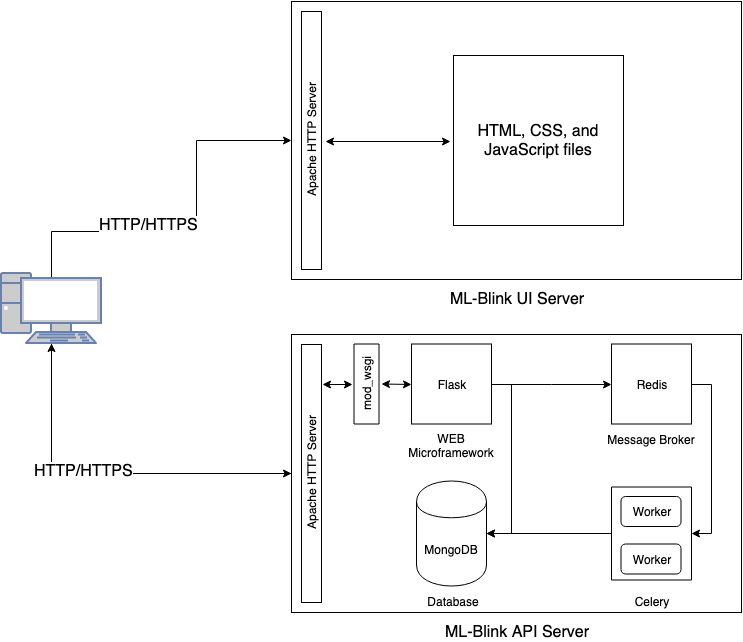
\includegraphics[
        width=\textwidth,
        height=\textheight,
        keepaspectratio
  ]{report/images/ml-blink-architecture.png}
  \caption{Summary of how the \mlblinkui and the \mlblinkapi interact with each other when used by a client depicted by a computer in this scenario.}
  \label{fig:ml-blink-architecture}
\end{figure}
\subsection{Server Architecture} \label{subsect:case-study:arch:server}

The \mlblinkapi runs in its own server using \ubuntu and it is written in \python. It closely follows the Representational State Transfer (\rest) software architecture, where applications provide consistent interface semantics (usually create, read, update, and delete for each resource) rather than arbitrary interfaces. Additionally, the \rest interactions are ``stateless'' in the sense that a response provided by an application is dependent on the parameters it receives, not in the current state of it \cite{web:w3:rest}. \newline

To aid in the design of a \rest application, the \mlblinkapi is build on top of the Flask microframework \cite{software:flask}, which provides useful methods and abstractions to create web services that follow \rest conventions with minimal effort. The \mlblinkapi is served using the Apache HTTP Server in conjunction with \texttt{mod\_wsgi}; an an Apache HTTP Server module that enables Apache to serve Flask applications. \newline

The majority of the data produced by the \mlblinkui usually consists of a structure of nested objects, as a result MongoDB was selected as the database for persisting data in the \mlblinkapi. Additionally, since the UI uses Asynchronous JavaScript and XML (AJAX) requests to communicate with the server, the \mlblinkapi defines Cross--Origin Resource Sharing (CORS) rules to restrict that only the domain in which the \mlblinkui is being served from can access the server's resources; such as when retrieving a mission setup, or creating a mission along with its achieved accuracy and other attributes. \newline

Finally, the \mlblinkapi uses the Celery distributed task queue \cite{software:celery} with Redis as a message broker in order to execute time--consuming tasks in the background without blocking the API. The Celery distributed task queue was also selected as it comes with an API that allows to execute background tasks concurrently on multiple processors.
\subsection{Client Architecture} \label{subsect:case-study:arch:client}

The \mlblinkui is entirely written in JavaScript. Since the UI allows for quite complex user interaction, the \texttt{Vue.js} framework \cite{software:vue} -- an open-source JavaScript framework for building user interfaces -- is used as the view layer to develop the user interface. Additionally, the application uses the Vue Command Line Interface (Vue CLI) to make local development, scaffolding, and deployment easier. \newline

The \mlblinkui communicates with the \mlblinkapi through AJAX calls that closely follow the REST standard, as pointed out in section \ref{subsect:case-study:arch:server}. These AJAX calls request the required data and resources to show to the user in the UI, as well as send data created by the user while using the UI to the \mlblinkapi to be persisted in the database. \newline

Lastly, similar to the \mlblinkapi, the \mlblinkui is hosted in its own server running in \ubuntu, and it uses the Apache HTTP server to serve requested resources as well.

% Implementation

% ML-Blink UI
% > Image matching
% > ROI
% > Using correlation to compute accuracy
% > Using image subtraction to compute accuracy

% ML-Blink API
% > Explicit representation
% > Implicit representation
% > Active set
% > Crawling potential candidates
% > Selecting candidate
% > Potential anomalies